\chapter{Application Performance}
A short study of the rendering performance of our solution is conducted to verify the targeted 10fps for a "simple image". We define the fourth iterate of \textsc{Gosper's flowsnake}, rendered with no rounding as a "simple image" and conduct the following benchmarks using its \gls{lsys}, invoked as

\begin{lstlisting}[language=bash]
$ ./pfcrender lsys  --rules "L L L+R++R-L--LL-R+ R -L+RR++R+L--L-R + + - - _ _ ~ ~" --sw 2 --sl 10  --it 4 --rd 0 --ia -60 --a 60
\end{lstlisting}
\begin{figure}[ht]
	\centering
	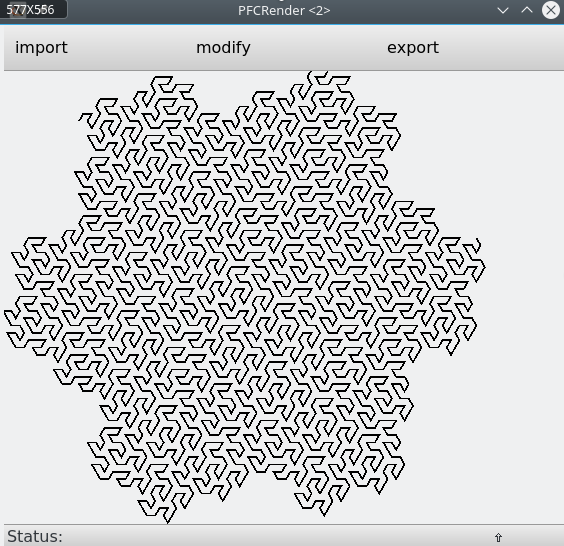
\includegraphics[width=0.8\textwidth]{simp_flosnek}
\end{figure}

Measurements are taken in an Archlinux virtual machine on an Intel Xeon E5 system at 3.5Ghz clock frequency and the program is compiled in release configuration with the following optimization flags
\begin{lstlisting}
-O3 -DNDEBUG -flto=full 
\end{lstlisting}

\section{Batch Mode Execution Timing}\label{sec:batchperf}
The following measurements are taken using the following shell command based on the Unix \cmd{time} utility. It executes the application 100 times in batch mode and averages the reported execution times of each run.
\begin{lstlisting}
for i in {1..100}; do { time ( ./pfcrender --clear --batch lsys  --rules "L L L+R++R-L--LL-R+ R -L+RR++R+L--L-R + + - - _ _ ~ ~" --sw 2 --sl 10  --it 4 --rd 0 --ia -60 --a 60 ) } 2>&1 |tail -1| sed 's/.*  //'|cut -d" " -f1|cut -c1-4 ;done | awk '{ total += $1; count++ } END { print total/count }'
\end{lstlisting}

We compare the runtime executing different plugins in batch mode.
\begin{table}[h]
	\centering
	\begin{tabular}{r|l}
		Testcase & Application runtime[ms]\\\hline\hline
		Import only & 68.7\\\hline
		Import \& SVG output & 73.3\\\hline
		Import \& PDF output & 76.1
	\end{tabular}
	\caption{Execution timings for the 4th iterate of \textsc{Gosper's flowsnake}}
	\label{tab:batchmeas}
\end{table}

It is apparent from these results, that the actual execution of a plugin's routine has a low impact on application runtime when the model is simple, as timings are dominated by application startup overhead. Irrespective of this effect, the proposed 100ms rendering time target is reached, even though SVG and PDF use the slow QPainter drawing engine and access the filesystem.

\section{GUI Rendering Timing}
As the timing of application startup and input plugin execution is known from the measurements in section \ref{sec:batchperf}, we benchmark the timing from triggering a model change to finishing of the rendering.

In order to obtain execution timings within the code, a test case was built into the sources, which can be found in \gls{git} as tagged commit \cmd{benchmark\_17-2-12}.

It starts a timer, feeds a pre-iterated model string of \textsc{Gosper's flowsnake} to the model and waits for the \class{QNanoCurvePainter} to signal completion of its \code{paint()} method, after which the rendering is finished. 

Reporting completion via the Signals/Slots mechanism is not a precise way of timing measurement as signal notifications are asynchronously handled by the \gls{gui} event loop. This can introduce additional delays to the timing, depending on when application control flow returns to it. As we are interested in the lower bound of performance though, this is not an issue here.

Timings are printed to console and - as shown in figure \ref{fig:guimeas} - consistently below 30ms. The total \gls{gui} rendering time, consisting of import from \gls{lsys} as measured in table \ref{tab:batchmeas} (70ms) and this rendering time is thus confirmed to be just below the 100ms mark required in figure \ref{fig:directreq}.

\begin{figure}
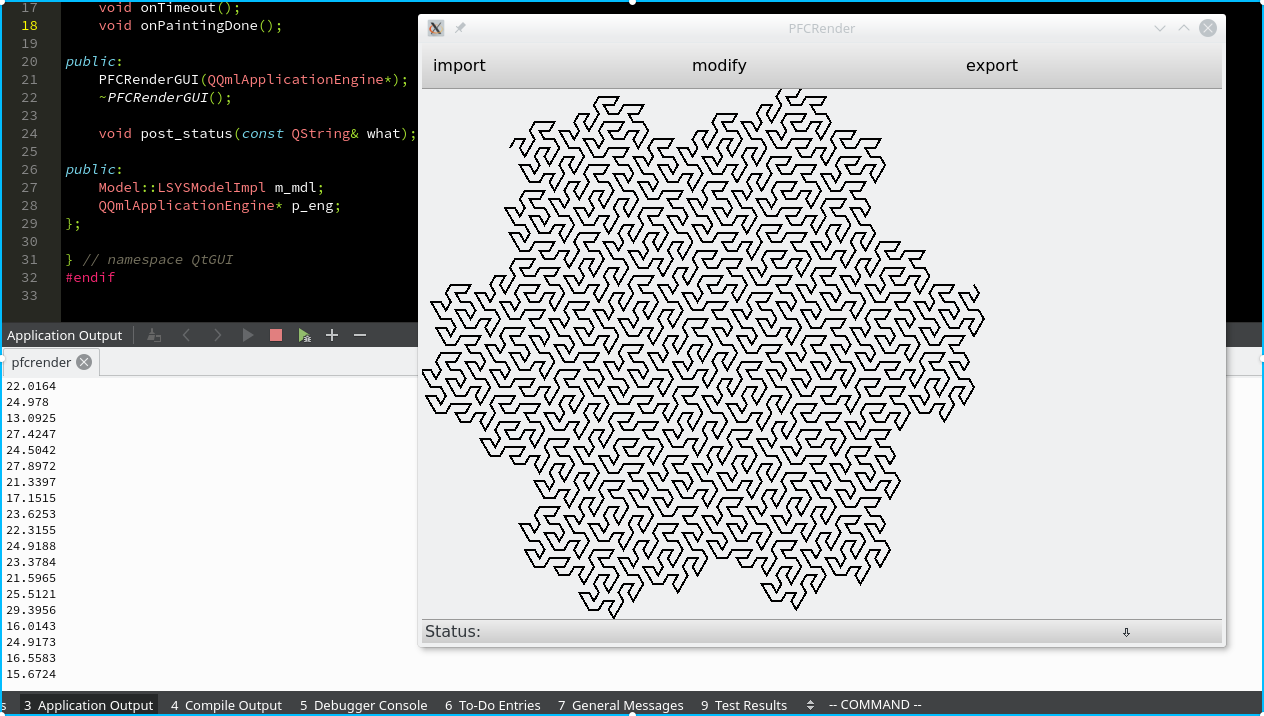
\includegraphics[width=\textwidth]{guimeasurement}
\caption{\gls{gui} Rendering Cycle Measurement}
\label{fig:guimeas}
\end{figure}
